% Note that if you want something in single space you can go back and
% forth between single space and normal space by the use of \ssp and
% \nsp.  If you want doublespacing you can use \dsp.  \nsp is normally
% 1.5 spacing unless you use the doublespace option (or savepaper
% option)
%
%(FORMAT) usually you *don't* want to mess with the spacing for your
%(FORMAT) final version.  If you think/know that the thesis template
%(FORMAT) and/or thesis style file is incorrect/incomplete, PLEASE
%(FORMAT) contact the maintainer.  THANK YOU!!!

\chapter{THE ALGORITHM}
\label{chap:thealgorithm}
% By labeling the chapter, I can refer to it later using the
% label. (\ref{chap:thealgorithm}, \pageref{chap:thealgorithm}) Latex will take care
% of the numbering.

In this chapter we will take a look at the details of the algorithm that we have been talking in the previous chapters. This is the algorithm which finds out the actual intersection points among a set of line segments in a two dimensional space. Though this algorithm is primarily for a two dimensional space.  It can be easily extended for 3 or n dimensional space with slight modification. Right now we will be limiting ourselves to 2 dimensional primary version of the algorithm.

\section{Data structures}

The algorithm requires several data structures. The first one is called as the event queue which stores all the events. We will denote the event queue by `Q'. The data structure that represents the `Q' should basically support the operations for fetching (removing) the next event so that it can be processed. This next event that needs to be fetched should be the highest event point below the sweep line. So the event points should be stored efficiently such that the events are fetched in right order with least time. If two event points are on the same horizontal line then the left event point is returned first. So imagine that the horizontal sweep line in inclined a bit downwards on the left side (Figure.~\ref{fig10} \cite{TEXTBOOK}) so that it reaches the left event points first than the right event points falling on the same horizontal line. 
\begin{figure}[ht]
  \begin{center}
   	\fbox{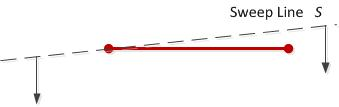
\includegraphics[width=4in, height=1.5in]{Figures/Figure10}}
  \end{center}
  \centering
	\parbox{4in}{\caption{Sweep line passing through a horizontal line. Adapted from Source: M. DE BERG, M. VAN KREVELD, M. OVERMARS, AND O. SCHWARZKOPF, \textbf{\textit{Computational Geometry- Algorithms and Applications}}, Springer Verlag, Berlin, Germany, 2000, ch. 2, pp. 19-29.} \label{fig10}} 
\end{figure}

This data structure should also support the insertion operation because there are some event points like the intersection points, which are computed dynamically, and which needs to be inserted into the event queue. Also many times it may happen that the two event points coincide such that the end points of two event points are the same. In such case we assume that the event point is the same. So the event queue should also support operation to tell if the event point already exists in the queue. It is important to remember that the event queue `Q' should support all these operations while maintaining the integrity of the queue. To summarize the event queue `Q' should support the below operations.
\begin{enumerate}
	\item Insertion
	\item Deletion
	\item Detecting if an event point already exists in the queue.
\end{enumerate}

\section{Implementation}

We will implement the event queue as an AVL tree (Figure.~\ref{fig11} \cite{TEXTBOOK}). We decided not to use heap data structure to implement the queue as this data structure also needs to support the operation of finding whether a given event point is already present in the `Q' which is not possible in the heap. We will define an order a on the event points that represents the order in which they will be handled. Thus if A and B are two event points then we have $A \alpha B$ if and only if A$_y$ $>$ B$_y$ holds or A$_y$ $=$ B$_y$ and A$_x$ $<$ B$_x$ holds. With each event point M we will store the segments whose starting end point is M.
\begin{figure}[ht]
  \begin{center}
   	\fbox{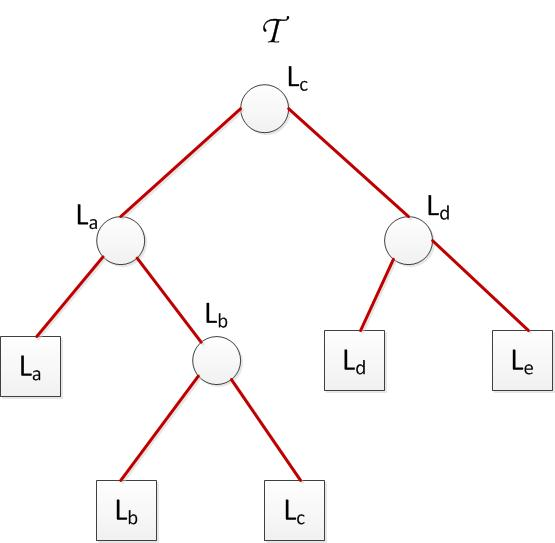
\includegraphics[width=4.5in, height=2.25in]{Figures/Figure11}}
  \end{center}
  \centering
	\parbox{4.5in}{\caption{An AVL tree representing a status structure. Adapted from Source: M. DE BERG, M. VAN KREVELD, M. OVERMARS, AND O. SCHWARZKOPF, \textbf{\textit{Computational Geometry- Algorithms and Applications}}, Springer Verlag, Berlin, Germany, 2000, ch. 2, pp. 19-29.} \label{fig11}} 
\end{figure}	

\section{Status Structure $\tau$}

Second, we need to maintain the status of the algorithm. This data structure is used to maintain the status of lines intersecting the sweep line in an ordered sequence. This data structure is denoted by `$\tau$'. The status structure is used to determine the neighbors of a given segment so that they can be tested for intersection. This status structure must be dynamic as segments continuously start or stop to intersect the sweep line and thus the data structure needs to be maintained accordingly at real time. Whenever a line segments `L' starts to intersect the sweep line `S' it is inserted into `$\tau$' and whenever the line segment stops intersecting `S' then it is deleted from `$\tau$'. The line segment must be inserted at appropriate position into `$\tau$' since it will used to determine the intersection tests with the neighbors. We will use an AVL tree to implement the status structure `$\tau$' (Figure.~\ref{fig12} \cite{TEXTBOOK}).
\begin{figure}[ht]
  \begin{center}
   	\fbox{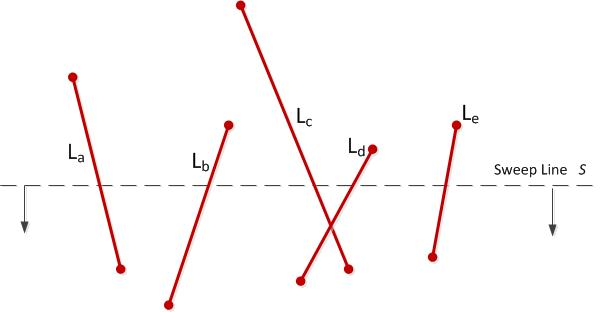
\includegraphics[width=6in, height=3in]{Figures/Figure12}}
  \end{center}
  \centering
	\parbox{6in}{\caption{Actual lines represented by a status structure. Adapted from Source: M. DE BERG, M. VAN KREVELD, M. OVERMARS, AND O. SCHWARZKOPF, \textbf{\textit{Computational Geometry- Algorithms and Applications}}, Springer Verlag, Berlin, Germany, 2000, ch. 2, pp. 19-29.} \label{fig12}} 
\end{figure}

Thus we store the segments intersecting the sweep line ordered in the leaves of the AVL tree `$\tau$'. The left-to-right order of the segments along the sweep line corresponds to the left-to-right order of the leaves in `$\tau$'. At each internal node we must store some data that will guide the search down to the leaves of the tree. At each internal node we store the rightmost segment in the left subtree. Storing of the line segments at the leaf node may sound like some redundant information as this could also be achieved by storing it only in the internal nodes. But it is conceptually simpler to think that the internal nodes should not store the data but only values to guide the search. Also storing of the segments at the leaf node makes the data structure more simple and easy to understand visually. Suppose we search in `$\tau$' for some segment immediately to the right of some point `P' that lies on the sweep line. At each internal node `V' we simply test whether `P' lies to the left of right of the segment stored at `V' and we navigate to the left or right depending on the result, eventually ending up in a leaf node. Either this leaf or the leaf immediately to the right of it is the segment that we are searching for. Similarly we can store the segment immediately to the left of `P' or the segment containing `P'. Thus each update and neighbor search operation takes {/it O}(log n) time. Please note this time complexity as further we will introduce some changes to the data structure `$\tau$' such that it will reduce this time.

\section{Formal Algorithm}

The formal algorithm as stated in the text book [14] is as follows-
\noindent
Algorithm FindIntersections(L) \newline
{\it Input:} A set S of line segments in the plane \newline
{\it Output:} The set of intersection points among the segments in L, with for each intersection point the segments that contain it.
\begin{enumerate}
	\item Initialize an empty queue Q. Next, insert the segment endpoints into Q; when an upper endpoint is inserted, the corresponding segment should be stored with it.
	\item Initialize an empty status structure $\tau$.
	\item while Q is not empty
	\item \hspace*{2em} do Determine the next event point P in Q and delete it.
	\item \hspace*{4em} HandleEventPoint(P)
\end{enumerate}

We have already seen how events are handled: at endpoints of segments we have to insert or delete segments from the status structure $\tau$, and at intersection points we have to change the order of two segments. In both cases we also have to do intersection tests between segments that become neighbors after the event (Figure.~\ref{fig131} \cite{TEXTBOOK}). In degenerate cases, where several segments are involved in one event point, the details are a little bit tricky. The next procedure describes how to handle event points correctly.

\noindent
HandleEventPoint(P)
\begin{enumerate}
	\item Let {\it U}(P) be he set of segments whose upper endpoint is P; these segments are stored with the event point P. (For horizontal segments, the upper endpoint is by definition the left endpoint.)
	\item Find all segments stored in $\tau$ that contain P; they are adjacent in $\tau$ (Figure.~\ref{fig132} \cite{TEXTBOOK}). Let L(P) denote the subset of segments found whose lower endpoint is P, and let C(P) denote the subset of segments found that contain P in their interior.
	\item if L(P) U {\it U}(P) U C(P) contains more than one segment
	\item \hspace*{2em} then Report P as an intersection, together with L(P), U(P), and C(P)
	\item Delete the segments in L(P) U C(P) from $\tau$.
	\item Insert the segments in {\it U}(P) U C(P) into $\tau$. The order of the segments in $\tau$ should correspond to the order in which they are intersected by a sweep line just below P. If there is a horizontal segment, it comes last among all segments including P.
	\item (* Deleting ad re-inserting the segments of C(P) reverses their order. *)
	\item if {\it U}(P) U C(P) = $\phi$
	\item then Let S$_l$ and S$_r$ be the left and right neighbors of P in $\tau$.
	\item \hspace*{2em} FindNewEvent(S$_l$, S$_r$, P)
	\item else Let S` be the leftmost segment of U(P) U C(P) in $\tau$
	\item \hspace*{2em} Let S$_l$ be the left neighbor of S` in $\tau$
	\item \hspace*{2em} FindNewEvent(S$_l$, S`, P)
	\item \hspace*{2em} Let S'' be the rightmost segment of U(P) U C(P) in $\tau$
	\item \hspace*{2em} Let S$_r$ be the rightmost neighbor of S'' in $\tau$
	\item \hspace*{2em} FindNewEvent(S'', S$_r$, P)
\end{enumerate}
\begin{figure}[ht]
  \begin{center}
   	\fbox{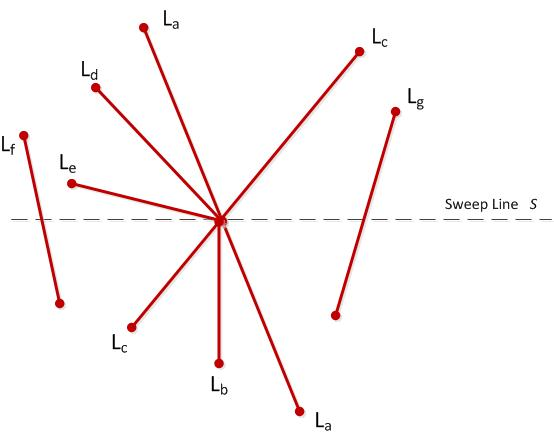
\includegraphics[width=4in, height=2in]{Figures/Figure13-1.jpg}}
  \end{center}
  \centering
	\parbox{4in}{\caption{A snapshot of an instance of sweep line in a running algorithm. Adapted from Source: M. DE BERG, M. VAN KREVELD, M. OVERMARS, AND O. SCHWARZKOPF, \textbf{\textit{Computational Geometry- Algorithms and Applications}}, Springer Verlag, Berlin, Germany, 2000, ch. 2, pp. 19-29.} \label{fig131}} 
\end{figure}
\begin{figure}[ht]
  \begin{center}
   	\fbox{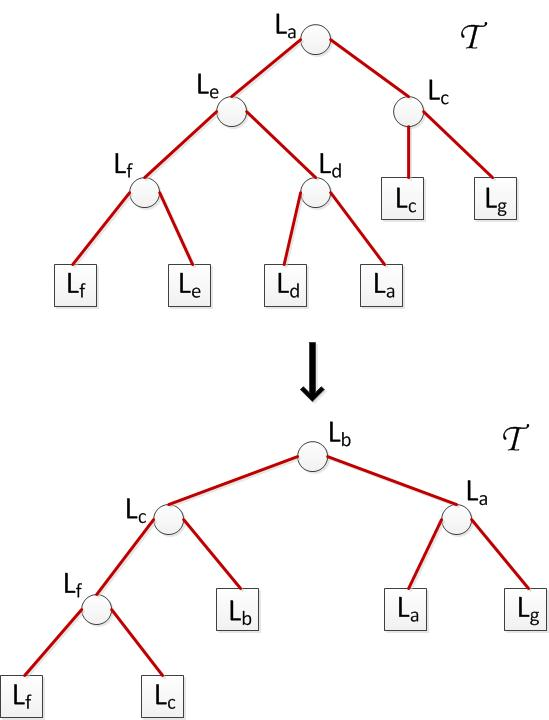
\includegraphics[width=4in, height=4.5in]{Figures/Figure13-2.jpg}}
  \end{center}
  \centering
	\parbox{4in}{\caption{A snapshot of a status structure in a running algorithm. Adapted from Source: M. DE BERG, M. VAN KREVELD, M. OVERMARS, AND O. SCHWARZKOPF, \textbf{\textit{Computational Geometry- Algorithms and Applications}}, Springer Verlag, Berlin, Germany, 2000, ch. 2, pp. 19-29.} \label{fig132}} 
\end{figure}

Note that in lines 8-16 we assume that Sl and Sr actually exists. If they do not exist the corresponding steps should obviously not be performed. The procedures for finding the new intersections are easy: they simply test two segments for intersection. The only thing we need to be careful about is, when we find an intersection, whether this intersection had already been handled earlier or not. When there are no horizontal segments, then the intersection has not been handled yet when the intersection point lies below the sweep line. But how should we deal with horizontal segments? Recall our convention that events with the same y- coordinate are treated from left to right. This implies that we are still interested in intersection points lying left to right of the current event point. Hence the procedure FindNewEvent is defined as follows.

\noindent
FindNewEvent(S$_l$, S$_r$, P)
\begin{enumerate}
	\item if S$_l$ and S$_r$ intersect below the sweep line, or on it and to the right of the current event point P, and the intersection is not yet present as an event in Q.
	\item \hspace*{2em} then Insert the intersection point as an event into Q.
\end{enumerate}
	
The algorithm that we just presented is output sensitive algorithm. This is a very important point as the algorithm time complexity depends not only on the input to the algorithm but it also depends on the output. In our case the output is the total number of intersection points. The pseudo code of the implemented algorithm is provided in Appendix~B.

\section{Time Complexity}

The total running time of the algorithm is {\it O}(( n + m ) log n) where n is the input size and m is the total number of intersection points. One intersection point can consists of a large number of segments, namely in the case where many segments intersect in a common point.

At the very beginning of the algorithm the event queue Q is constructed which takes {\it O}(n log n) time because we decided to implement the event queue as an AVL tree. The status structure initialization takes constant time. Then the algorithm starts out to handle each event point. There could be at the most three operations performed on each event
\begin{enumerate}
	\item The event itself is deleted from the event queue �Q� in step 5 of the algorithm. This will take {\it O}(log n) time each.
	\item There can be one or two calls to FindNewEvent which may cause at most two new events to be added to the event queue. This would also take {\it O}(log n) time each.
\end{enumerate}

We also perform the operations of inserting, deletion and finding neighbor on the status structure �$\tau$� that should take {\it O}(log n) time each. These number of operations are linear in the number m(p) := card(L(p) U  {\it U}(p) U  c(p)), over all event points p, by m, the running time of the algorithm is {\it O}(m log n). It is clear that m = {\it O}(n + k) where k is the output which is the total number of intersection points \cite{TEXTBOOK}. Also please note that the insertion, deletion and finding nearest neighbor in an AVL tree taken {\it O}(log n) time. The contribution of this research is to optimize the time required to compute the nearest neighbor which is one of the most frequent operation performed by the algorithm.
